\documentclass[]{article}

\usepackage{hyperref}

\usepackage{tikz}		% for grids

\title{HPCA-PC Exercise Sheet 2 --- Group 1}
\author{
	Mariia Isaeva\\
	\texttt{7910764}	\\
	\href{mailto:s6047802@stud.uni-frankfurt.de}{s6047802@stud.uni-frankfurt.de}
	\and
	Luiz Augusto da Silva Feitosa	\\
	\texttt{7890756}	\\
	\href{mailto:s1506025@stud.uni-frankfurt.de}{s1506025@stud.uni-frankfurt.de}
	\and
	Joshua Spingler\\
	\texttt{8243375}	\\
	\href{mailto:s7457265@stud.uni-frankfurt.de}{s7457265@stud.uni-frankfurt.de}
	\and
	Tim Wolf\\
	\texttt{7416419}	\\
	\href{mailto:s9677570@stud.uni-frankfurt.de}{s9677570@stud.uni-frankfurt.de}
}
\date{}

\begin{document}

\maketitle

\section*{Conway’s Game of Life}
\subsection*{Exercise 1.1: Design of the Cellular Automaton}
\subsection*{Exercise 1.2: Implement Conway’s Game of Life}
\subsection*{Exercise 1.3: Implement a Command Line Interface}
	\subsubsection*{Starting cell of multi-cell figures at the grid position (x,y)}
	\textcolor{red}{Explanation --- WORK IN PROGRESS (LUIZ)}

\begin{center}
	% Glider
	\begin{minipage}{0.32\textwidth}
		\centering
		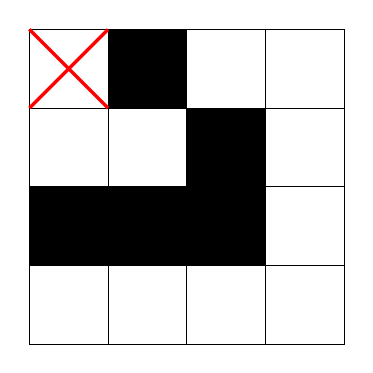
\begin{tikzpicture}
			\foreach \y in {0,...,3} {
				\foreach \x in {0,...,3} {
					\node[draw, minimum size=1cm] at (\x,-\y) {};
				}
			}
			\node[draw, minimum size=1cm, fill=black] at (1,0) {};
			\node[draw, minimum size=1cm, fill=black] at (2,-1) {};
			\node[draw, minimum size=1cm, fill=black] at (0,-2) {};
			\node[draw, minimum size=1cm, fill=black] at (1,-2) {};
			\node[draw, minimum size=1cm, fill=black] at (2,-2) {};
			
			\draw[red, very thick] (-0.5,0.5) -- (0.5,-0.5);
			\draw[red, very thick] (-0.5,-0.5) -- (0.5,0.5);
		\end{tikzpicture}
		\\[0.3cm]
		\textbf{Glider}
	\end{minipage}
	\hfill
	%Toad
	\begin{minipage}{0.32\textwidth}
		\centering
		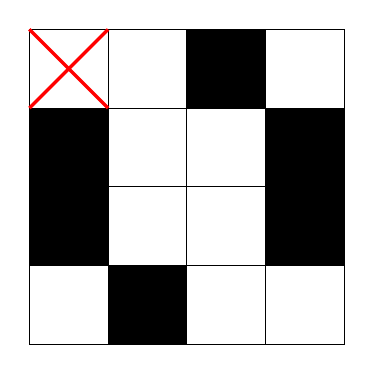
\begin{tikzpicture}
			\foreach \y in {0,...,3} {
				\foreach \x in {0,...,3} {
					\node[draw, minimum size=1cm] at (\x,-\y) {};
				}
			}
			\node[draw, minimum size=1cm, fill=black] at (2,0) {};
			\node[draw, minimum size=1cm, fill=black] at (0,-1) {};
			\node[draw, minimum size=1cm, fill=black] at (0,-2) {};
			\node[draw, minimum size=1cm, fill=black] at (1,-3) {};
			\node[draw, minimum size=1cm, fill=black] at (3,-1) {};
			\node[draw, minimum size=1cm, fill=black] at (3,-2) {};
			
			\draw[red, very thick] (-0.5,0.5) -- (0.5,-0.5);
			\draw[red, very thick] (-0.5,-0.5) -- (0.5,0.5);
		\end{tikzpicture}
		\\[0.3cm]
		\textbf{Toad}
	\end{minipage}
	\hfill
	% Beacon
	\begin{minipage}{0.32\textwidth}
		\centering
		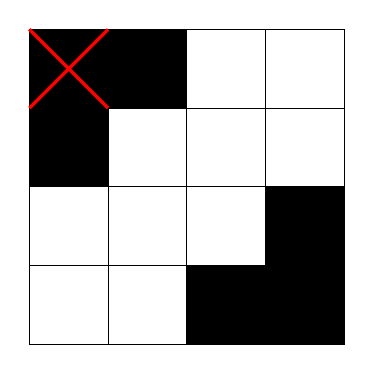
\begin{tikzpicture}
			\foreach \y in {0,...,3} {
				\foreach \x in {0,...,3} {
					\node[draw, minimum size=1cm] at (\x,-\y) {};
				}
			}
			\node[draw, minimum size=1cm, fill=black] at (0,0) {};
			\node[draw, minimum size=1cm, fill=black] at (1,0) {};
			\node[draw, minimum size=1cm, fill=black] at (0,-1) {};
			\node[draw, minimum size=1cm, fill=black] at (3,-2) {};
			\node[draw, minimum size=1cm, fill=black] at (2,-3) {};
			\node[draw, minimum size=1cm, fill=black] at (3,-3) {};
			
			\draw[red, very thick] (-0.5,0.5) -- (0.5,-0.5);
			\draw[red, very thick] (-0.5,-0.5) -- (0.5,0.5);
		\end{tikzpicture}
		\\[0.3cm]
		\textbf{Beacon}
	\end{minipage}
\end{center}



\subsection*{Exercise 1.4: Optimization Level and Compilation Settings}
\subsection*{Exercise 1.5: Simulation Time per Grid Size}

\end{document}
